\begin{figure}[H]
\centering
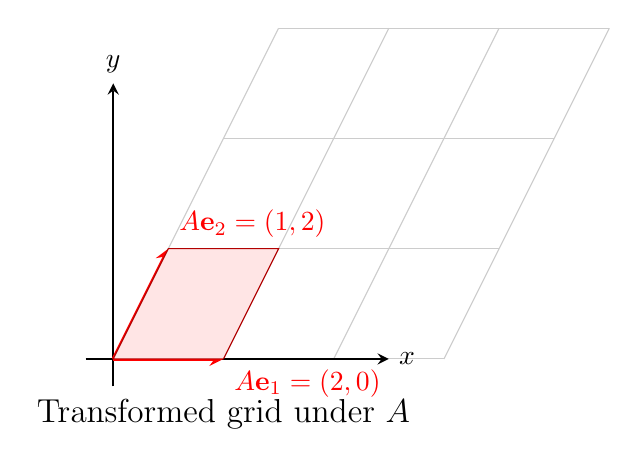
\begin{tikzpicture}[scale=0.7, >=stealth]
    % Transformation matrix vectors
    \def\a{2} % First column x
    \def\b{0} % First column y
    \def\c{1} % Second column x
    \def\d{2} % Second column y

    % Draw transformed grid
    \foreach \i in {0,...,3}{
        \draw[gray!40,thin] 
            ({\i*\a/1 + 0*\c}, {\i*\b/1 + 0*\d}) -- ({\i*\a/1 + 3*\c}, {\i*\b/1 + 3*\d});
        \draw[gray!40,thin]
            ({0*\a + \i*\c}, {0*\b + \i*\d}) -- ({3*\a + \i*\c}, {3*\b + \i*\d});
    }

    % Axes
    \draw[->,thick] (-0.5,0) -- (5,0) node[right] {$x$};
    \draw[->,thick] (0,-0.5) -- (0,5) node[above] {$y$};

    % Transformed basis vectors
    \draw[->,very thick,red] (0,0) -- (\a,\b) node[below right] {$A\mathbf{e}_1 = (2,0)$};
    \draw[->,very thick,red] (0,0) -- (\c,\d) node[above right] {$A\mathbf{e}_2 = (1,2)$};

    % Parallelogram showing the new unit cell
    \filldraw[fill=red!10, draw=red!70!black] 
      (0,0) -- (\a,\b) -- ({\a+\c},{\b+\d}) -- (\c,\d) -- cycle;

    % Label
    \node at (2, -1) {\large Transformed grid under $A$};
\end{tikzpicture}
\caption{The grid transformed by $A = \begin{bmatrix}2 & 1\\ 0 & 2\end{bmatrix}$.}
\end{figure}